\PassOptionsToPackage{unicode=true}{hyperref} % options for packages loaded elsewhere
\PassOptionsToPackage{hyphens}{url}
%
\documentclass[ignorenonframetext,]{beamer}
\usepackage{pgfpages}
\setbeamertemplate{caption}[numbered]
\setbeamertemplate{caption label separator}{: }
\setbeamercolor{caption name}{fg=normal text.fg}
\beamertemplatenavigationsymbolsempty
% Prevent slide breaks in the middle of a paragraph:
\widowpenalties 1 10000
\raggedbottom
\setbeamertemplate{part page}{
\centering
\begin{beamercolorbox}[sep=16pt,center]{part title}
  \usebeamerfont{part title}\insertpart\par
\end{beamercolorbox}
}
\setbeamertemplate{section page}{
\centering
\begin{beamercolorbox}[sep=12pt,center]{part title}
  \usebeamerfont{section title}\insertsection\par
\end{beamercolorbox}
}
\setbeamertemplate{subsection page}{
\centering
\begin{beamercolorbox}[sep=8pt,center]{part title}
  \usebeamerfont{subsection title}\insertsubsection\par
\end{beamercolorbox}
}
\AtBeginPart{
  \frame{\partpage}
}
\AtBeginSection{
  \ifbibliography
  \else
    \frame{\sectionpage}
  \fi
}
\AtBeginSubsection{
  \frame{\subsectionpage}
}
\usepackage{lmodern}
\usepackage{amssymb,amsmath}
\usepackage{ifxetex,ifluatex}
\usepackage{fixltx2e} % provides \textsubscript
\ifnum 0\ifxetex 1\fi\ifluatex 1\fi=0 % if pdftex
  \usepackage[T1]{fontenc}
  \usepackage[utf8]{inputenc}
  \usepackage{textcomp} % provides euro and other symbols
\else % if luatex or xelatex
  \usepackage{unicode-math}
  \defaultfontfeatures{Ligatures=TeX,Scale=MatchLowercase}
\fi
% use upquote if available, for straight quotes in verbatim environments
\IfFileExists{upquote.sty}{\usepackage{upquote}}{}
% use microtype if available
\IfFileExists{microtype.sty}{%
\usepackage[]{microtype}
\UseMicrotypeSet[protrusion]{basicmath} % disable protrusion for tt fonts
}{}
\IfFileExists{parskip.sty}{%
\usepackage{parskip}
}{% else
\setlength{\parindent}{0pt}
\setlength{\parskip}{6pt plus 2pt minus 1pt}
}
\usepackage{hyperref}
\hypersetup{
            pdftitle={geotopbricks},
            pdfauthor={Emanuele Cordano},
            pdfborder={0 0 0},
            breaklinks=true}
\urlstyle{same}  % don't use monospace font for urls
\newif\ifbibliography
\usepackage{color}
\usepackage{fancyvrb}
\newcommand{\VerbBar}{|}
\newcommand{\VERB}{\Verb[commandchars=\\\{\}]}
\DefineVerbatimEnvironment{Highlighting}{Verbatim}{commandchars=\\\{\}}
% Add ',fontsize=\small' for more characters per line
\usepackage{framed}
\definecolor{shadecolor}{RGB}{248,248,248}
\newenvironment{Shaded}{\begin{snugshade}}{\end{snugshade}}
\newcommand{\AlertTok}[1]{\textcolor[rgb]{0.94,0.16,0.16}{#1}}
\newcommand{\AnnotationTok}[1]{\textcolor[rgb]{0.56,0.35,0.01}{\textbf{\textit{#1}}}}
\newcommand{\AttributeTok}[1]{\textcolor[rgb]{0.77,0.63,0.00}{#1}}
\newcommand{\BaseNTok}[1]{\textcolor[rgb]{0.00,0.00,0.81}{#1}}
\newcommand{\BuiltInTok}[1]{#1}
\newcommand{\CharTok}[1]{\textcolor[rgb]{0.31,0.60,0.02}{#1}}
\newcommand{\CommentTok}[1]{\textcolor[rgb]{0.56,0.35,0.01}{\textit{#1}}}
\newcommand{\CommentVarTok}[1]{\textcolor[rgb]{0.56,0.35,0.01}{\textbf{\textit{#1}}}}
\newcommand{\ConstantTok}[1]{\textcolor[rgb]{0.00,0.00,0.00}{#1}}
\newcommand{\ControlFlowTok}[1]{\textcolor[rgb]{0.13,0.29,0.53}{\textbf{#1}}}
\newcommand{\DataTypeTok}[1]{\textcolor[rgb]{0.13,0.29,0.53}{#1}}
\newcommand{\DecValTok}[1]{\textcolor[rgb]{0.00,0.00,0.81}{#1}}
\newcommand{\DocumentationTok}[1]{\textcolor[rgb]{0.56,0.35,0.01}{\textbf{\textit{#1}}}}
\newcommand{\ErrorTok}[1]{\textcolor[rgb]{0.64,0.00,0.00}{\textbf{#1}}}
\newcommand{\ExtensionTok}[1]{#1}
\newcommand{\FloatTok}[1]{\textcolor[rgb]{0.00,0.00,0.81}{#1}}
\newcommand{\FunctionTok}[1]{\textcolor[rgb]{0.00,0.00,0.00}{#1}}
\newcommand{\ImportTok}[1]{#1}
\newcommand{\InformationTok}[1]{\textcolor[rgb]{0.56,0.35,0.01}{\textbf{\textit{#1}}}}
\newcommand{\KeywordTok}[1]{\textcolor[rgb]{0.13,0.29,0.53}{\textbf{#1}}}
\newcommand{\NormalTok}[1]{#1}
\newcommand{\OperatorTok}[1]{\textcolor[rgb]{0.81,0.36,0.00}{\textbf{#1}}}
\newcommand{\OtherTok}[1]{\textcolor[rgb]{0.56,0.35,0.01}{#1}}
\newcommand{\PreprocessorTok}[1]{\textcolor[rgb]{0.56,0.35,0.01}{\textit{#1}}}
\newcommand{\RegionMarkerTok}[1]{#1}
\newcommand{\SpecialCharTok}[1]{\textcolor[rgb]{0.00,0.00,0.00}{#1}}
\newcommand{\SpecialStringTok}[1]{\textcolor[rgb]{0.31,0.60,0.02}{#1}}
\newcommand{\StringTok}[1]{\textcolor[rgb]{0.31,0.60,0.02}{#1}}
\newcommand{\VariableTok}[1]{\textcolor[rgb]{0.00,0.00,0.00}{#1}}
\newcommand{\VerbatimStringTok}[1]{\textcolor[rgb]{0.31,0.60,0.02}{#1}}
\newcommand{\WarningTok}[1]{\textcolor[rgb]{0.56,0.35,0.01}{\textbf{\textit{#1}}}}
\usepackage{graphicx,grffile}
\makeatletter
\def\maxwidth{\ifdim\Gin@nat@width>\linewidth\linewidth\else\Gin@nat@width\fi}
\def\maxheight{\ifdim\Gin@nat@height>\textheight\textheight\else\Gin@nat@height\fi}
\makeatother
% Scale images if necessary, so that they will not overflow the page
% margins by default, and it is still possible to overwrite the defaults
% using explicit options in \includegraphics[width, height, ...]{}
\setkeys{Gin}{width=\maxwidth,height=\maxheight,keepaspectratio}
\setlength{\emergencystretch}{3em}  % prevent overfull lines
\providecommand{\tightlist}{%
  \setlength{\itemsep}{0pt}\setlength{\parskip}{0pt}}
\setcounter{secnumdepth}{0}

% set default figure placement to htbp
\makeatletter
\def\fps@figure{htbp}
\makeatother

%% EMOS rmarkdown/beamer header
%% Mark van der Loo (2016)
\usepackage{listings}
\usepackage{mdframed}
\usepackage{tikz}

\usetikzlibrary{arrows, positioning, decorations.pathreplacing} 
\usepackage{pgfplots}
\usepackage{color}


% CBS corporate light blue
\definecolor{corplightblue}{HTML}{00a1cd}
% CBS corporate dark blue
\definecolor{corpdarkblue}{HTML}{0058b8}

% set title colors
\setbeamercolor{frametitle}{fg=corpdarkblue}
\setbeamercolor{title}{fg=corpdarkblue}
\setbeamercolor{block title}{fg=corpdarkblue}

\setbeamerfont{normal text}{parent=structure}
% nicer, rounder font for title
\setbeamerfont{title}{series=\bfseries,parent=structure}
% frame titles in boldface
\setbeamerfont{frametitle}{series=\bfseries}
% block title font
\setbeamerfont{block title}{parent=structure}

% enumeration
\setbeamertemplate{itemize item}{\color{corpdarkblue}$\blacktriangleright$}
\setbeamertemplate{itemize subitem}{\color{corpdarkblue}$-$}
\setbeamercolor*{enumerate item}{fg=corpdarkblue}
\setbeamercolor*{enumerate subitem}{fg=corpdarkblue}
\setbeamercolor*{enumerate subsubitem}{fg=corpdarkblue}


\makeatletter
\newcommand\HUGE{\@setfontsize\Huge{50}{60}}
\makeatother    


% nicer, rounder font for title

\setbeamertemplate{title page}{
\begin{picture}(0,0)
\put(0,50){\usebeamerfont{title}{\textcolor{corpdarkblue}{\inserttitle}\par}}

\put(0,20){
\small Emanuele Cordano, Rendena100
}
\put(0,0){
\texttt{\small @ecor} | \texttt{\small github.com/ecor}
}


\put(150,-100){

\includegraphics[height=3cm]{resources/logo/logo_useR2019.png}
}
\end{picture}

}



\setbeamertemplate{frametitle}
{
  \begin{beamercolorbox}{frametitle}
  \vskip2.7ex\insertframetitle
  \end{beamercolorbox}
}


% remove the space-eating navigation symbols
\beamertemplatenavigationsymbolsempty

% convenience function to define rgb colors in tikz
\tikzset{xcolor/.code args={#1=#2}{
     \definecolor{mytemp}{rgb}{#2}
     \tikzset{#1=mytemp}
  }
}


\usebackgroundtemplate{
   \begin{picture}(0,0)
    \put(270, -273){%
      \raisebox{5mm}{\tiny useR2019, Toulouse,France }
\includegraphics[height=8mm]{resources/logo/logo_useR2019.png}
    }
\put(0,-273){

\includegraphics[height=7mm]{resources/logo/logo_geotop.jpeg}

\includegraphics[height=7mm]{resources/logo/logo_eurac.png}

\includegraphics[height=7mm]{resources/logo/logo_rendena100_textoutside_small.jpg}
}
\end{picture}
}


\newcommand{\la}[1]{\boldsymbol{#1}}

\title{geotopbricks}
\providecommand{\subtitle}[1]{}
\subtitle{An R Package for the Distributed Hydrological Model GEOtop}
\author{Emanuele Cordano}
\date{github/ecor / useR2019}

\begin{document}
\frame{\titlepage}

\begin{frame}{Who am I?}
\protect\hypertarget{who-am-i}{}

\begin{itemize}
\tightlist
\item
  Environmental engineer with hydraulic and hydrological background
  (more deterministic and physicall-based than statics!)
\item
  Some skills in programming and a R entusiast which I use to work with
  hydro-climatic data.
\item
  Find me as @ecor on GitHub
\item
  I'm self-employed and freelancer as www.rendena100.eu .\\
\item
  Author of several R-packages and p
\end{itemize}

\end{frame}

\begin{frame}[fragile]{Who are the other authors?}
\protect\hypertarget{who-are-the-other-authors}{}

\begin{itemize}
\tightlist
\item
  Hydrologist ,,, BLA
\item
  Author of several packages, including \texttt{geotop},\ldots{}
\end{itemize}

\end{frame}

\begin{frame}{Hydrology}
\protect\hypertarget{hydrology}{}

Scientific study of the movement, distribution, and quality of water on
Earth water cycle, water resources and environmental watershed
sustainability.

\begin{figure}
\centering
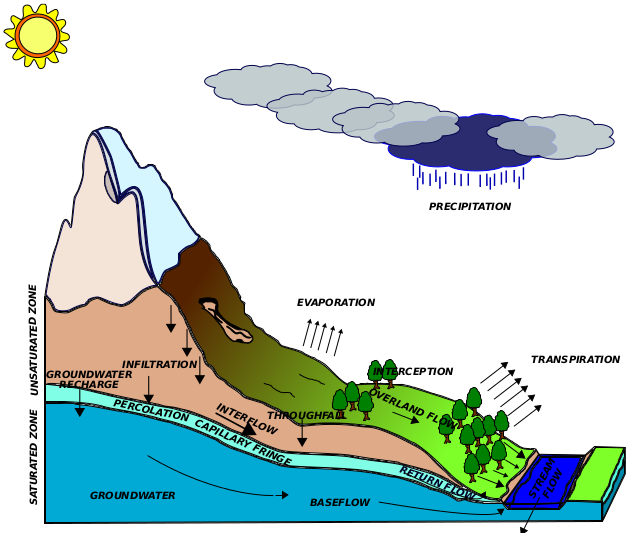
\includegraphics[width=0.5\textwidth,height=\textheight]{resources/images/geotop_landscape.png}
\caption{image}
\end{figure}

\end{frame}

\begin{frame}{Soil Water Balance}
\protect\hypertarget{soil-water-balance}{}

\end{frame}

\begin{frame}{GEOtop Hydrological Model}
\protect\hypertarget{geotop-hydrological-model}{}

GEOtop is an integrated hydrological model that simulates:

\begin{itemize}
\item water flow in the soil $\,\to\,$ Richards' eq (sub) + Kinematic eq (sur)
\item energy exchange with the atmosphere $\,\to\,$ full integration of equation
\end{itemize}

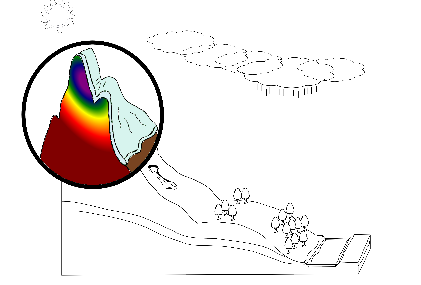
\includegraphics[width=0.2\textwidth,height=\textheight]{resources/images/geotop_snow.png}
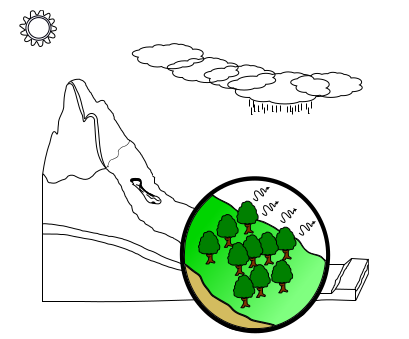
\includegraphics[width=0.2\textwidth,height=\textheight]{resources/images/geotop_vegetation.png}
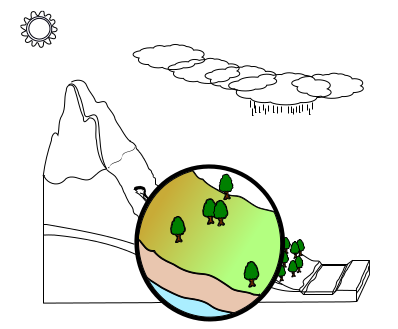
\includegraphics[width=0.2\textwidth,height=\textheight]{resources/images/geotop_infiltration.png}

\end{frame}

\begin{frame}{Hydrological Model}
\protect\hypertarget{hydrological-model}{}

\begin{itemize}
\tightlist
\item
  Input: meteo data, elevations, soil parameters
\item
  Output: snow cover, soil temperature, soil moisture
\end{itemize}

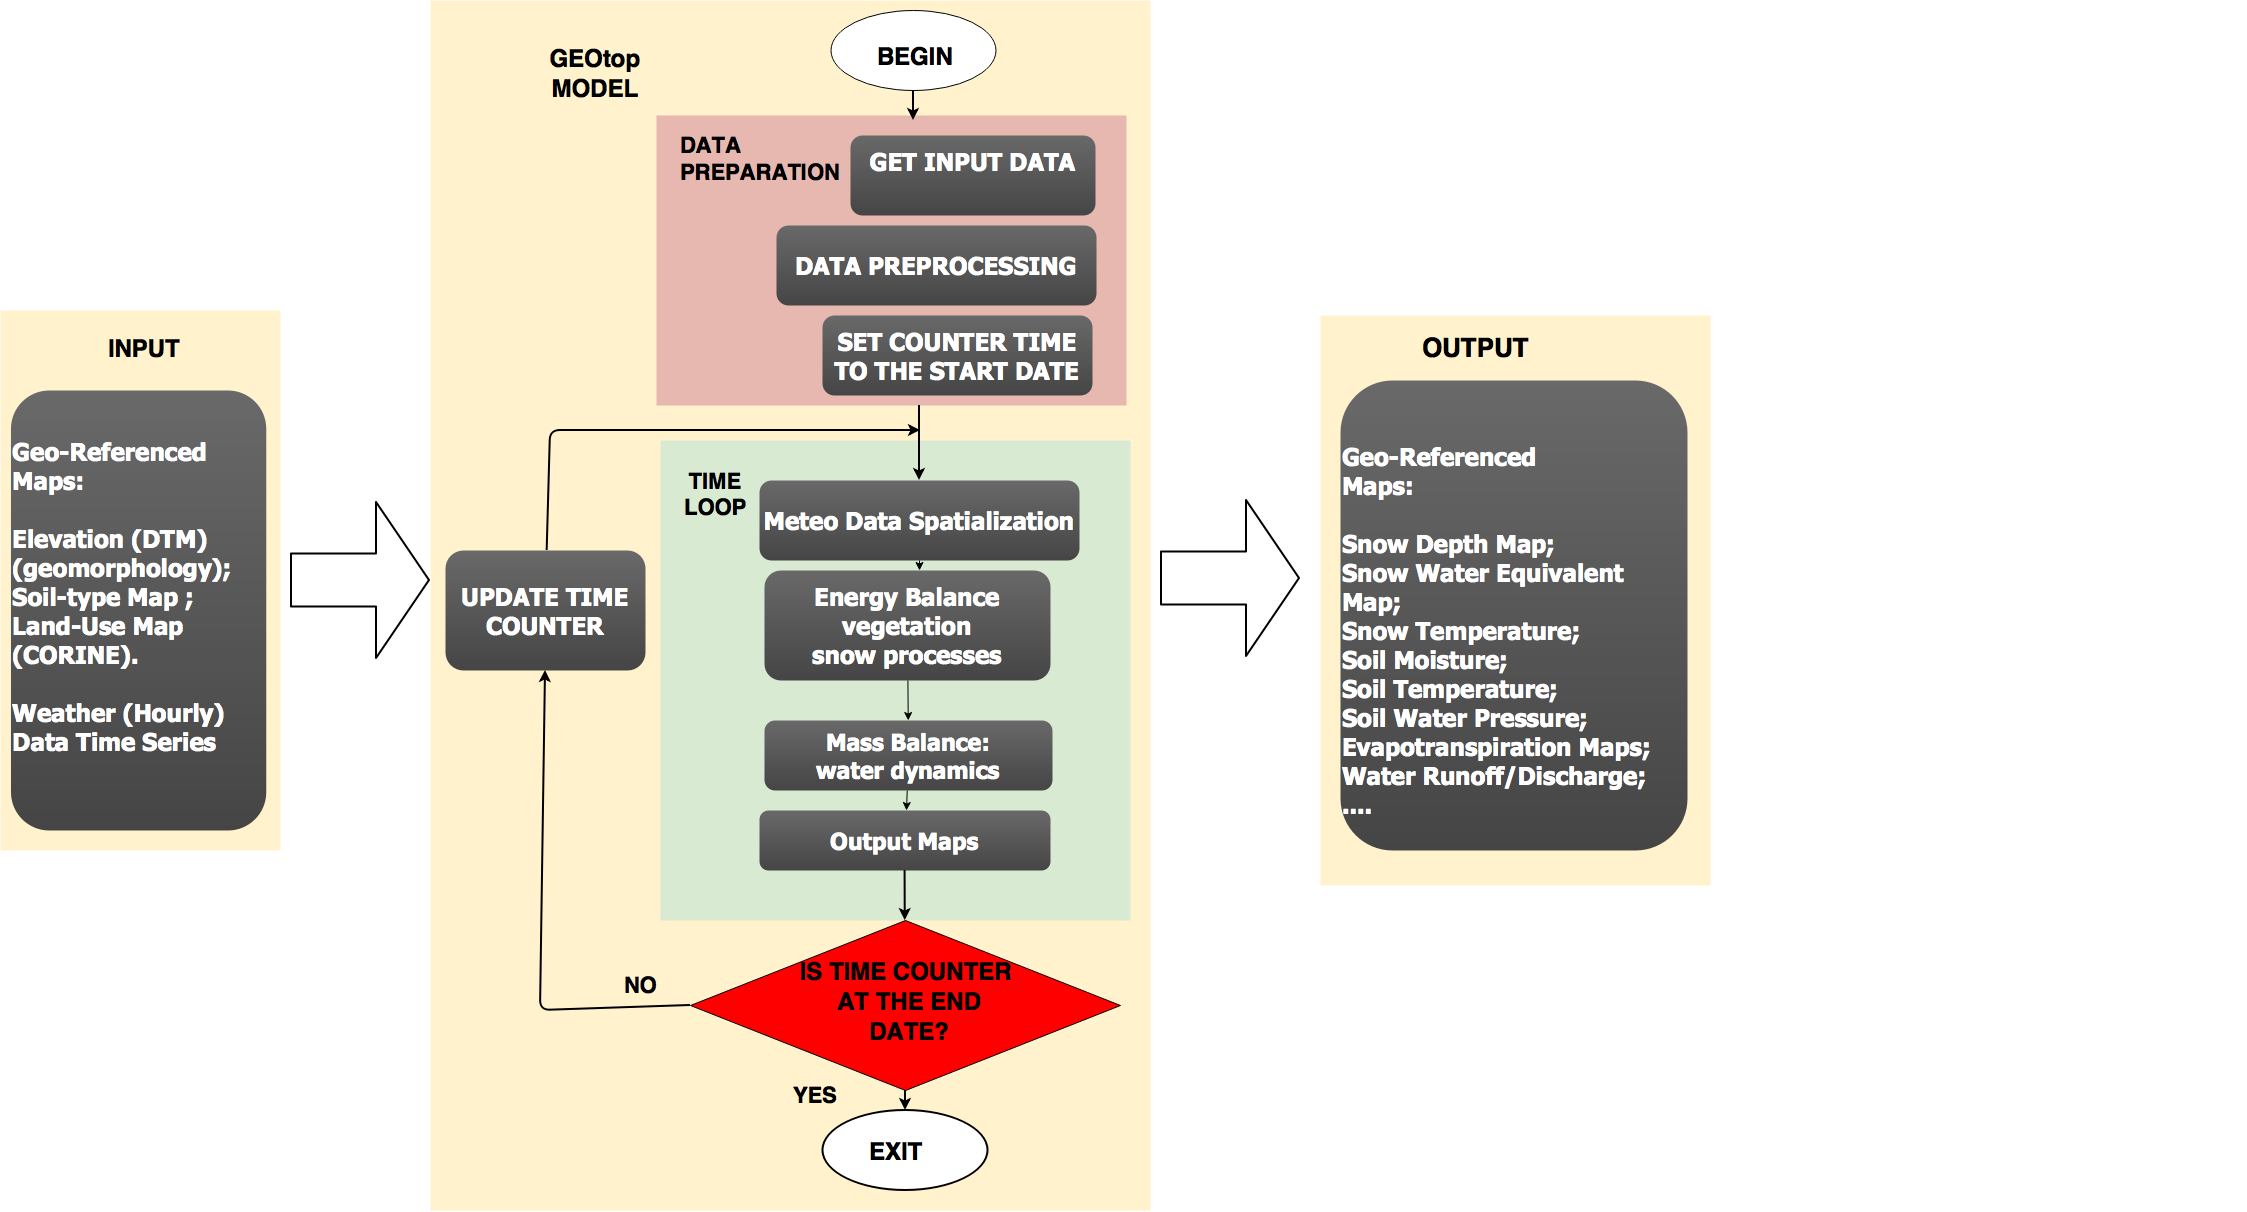
\includegraphics[width=0.9\textwidth,height=\textheight]{resources/images/geotop_revised.png}
\#\# GEOtop model\}\%\{Optional Subtitle

Water and energy budgets can be activated :

\begin{itemize}
\tightlist
\item
  one or the other \(\,\to\,\) simplification
\item
  both them together \(\,\to\,\) realistic
\end{itemize}

Two setup configurations : - \textbf{1D}: only vertical fluxes
\(\,\to\,\) mass and energy balance at local scale (only in one soil
column) - \textbf{3D}: vertical and lateral fluxes \(\,\to\,\) balances
at basin scale

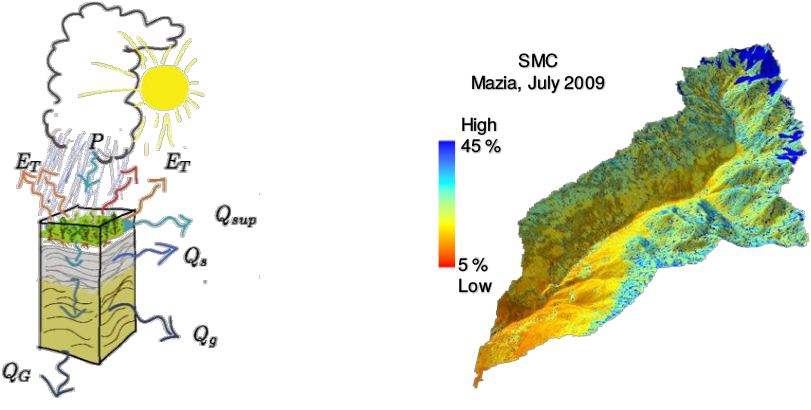
\includegraphics[width=0.9\textwidth,height=\textheight]{resources/images/geotop_ET_SWC.png}

Core components of GEOtop software packages are:

\begin{itemize}
\tightlist
\item
  written in C/C++
\item
  released in 2014 (version 2.0) as free open-source project, a
  re-engineering process is going to finish (version 3.0);
\item
  scientifically tested and published;
\item
  documented on GitHub repository:
  \emph{\url{http://geotopmodel.github.io/geotop/}}
\end{itemize}


\includegraphics[width=0.9\textwidth,height=\textheight]{resources/images/geotop_paper_2017.png}

\end{frame}

\begin{frame}{GEOtop external extensions}
\protect\hypertarget{geotop-external-extensions}{}

\textbf{Lorem ipsum} dolor sit amet, consectetur adipiscing elit, sed do
eiusmod tempor incididunt ut labore et dolore magna aliqua. Ut enim ad
minim veniam, quis nostrud exercitation ullamco laboris nisi ut aliquip
ex ea commodo consequat. Duis aute irure dolor in reprehenderit in
voluptate velit esse cillum dolore eu fugiat nulla pariatur. Excepteur
sint occaecat cupidatat non proident, sunt in culpa qui officia deserunt
mollit anim id est laborum

\end{frame}

\begin{frame}{GEOtop}
\protect\hypertarget{geotop}{}

placeholder

\end{frame}

\begin{frame}{GEOtop configuration File (geotop.inpts)}
\protect\hypertarget{geotop-configuration-file-geotop.inpts}{}

placeholder

\end{frame}

\begin{frame}[fragile]{GEOtop configuration File (geotop.inpts)}
\protect\hypertarget{geotop-configuration-file-geotop.inpts-1}{}

A GEOtop simulation is organized in a set of files within a directory.
This directory contains:

-\textbf{input files} (meteorological forcings, topography, land-use,
soil-type maps, initial conditions); \textbf{target information} (which
results are requested) ; - \textbf{observations}. Allthese information
are written in a file called \texttt{geotop.inpts}, which is a list of
\textbf{keyword-value} pairs:

\begin{verbatim}
InitDateDDMMYYYYhhmm    =   09/04/2014 18:00  
EndDateDDMMYYYYhhmm     =   01/01/2016 00:00 
[...] 
MeteoFile               =   "meteoB2_irr" 
PointOutputFile         =   "tabs/point" 
\end{verbatim}

\end{frame}

\begin{frame}{Simulation of soil water budget in an alpine site}
\protect\hypertarget{simulation-of-soil-water-budget-in-an-alpine-site}{}

GOtop is applied to estimate soil water content in two soil columns
below two hydro-meteorological stations (B2 and P2) located in Val
Mazia/Match, Malles Venosta/Mals Vinschgau, in South Tyrol, Italy (LOng
Term Reasearch Ecological Area, {[}\url{http://lter.eurac.edu/en}{]}).

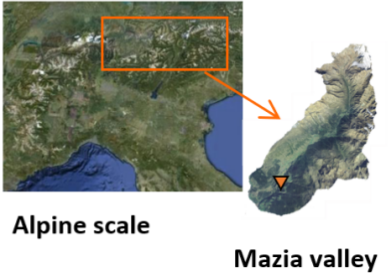
\includegraphics[width=0.4\textwidth,height=\textheight]{resources/images/mazia_2.png}

\end{frame}

\begin{frame}{Geotopbricks Graph}
\protect\hypertarget{geotopbricks-graph}{}

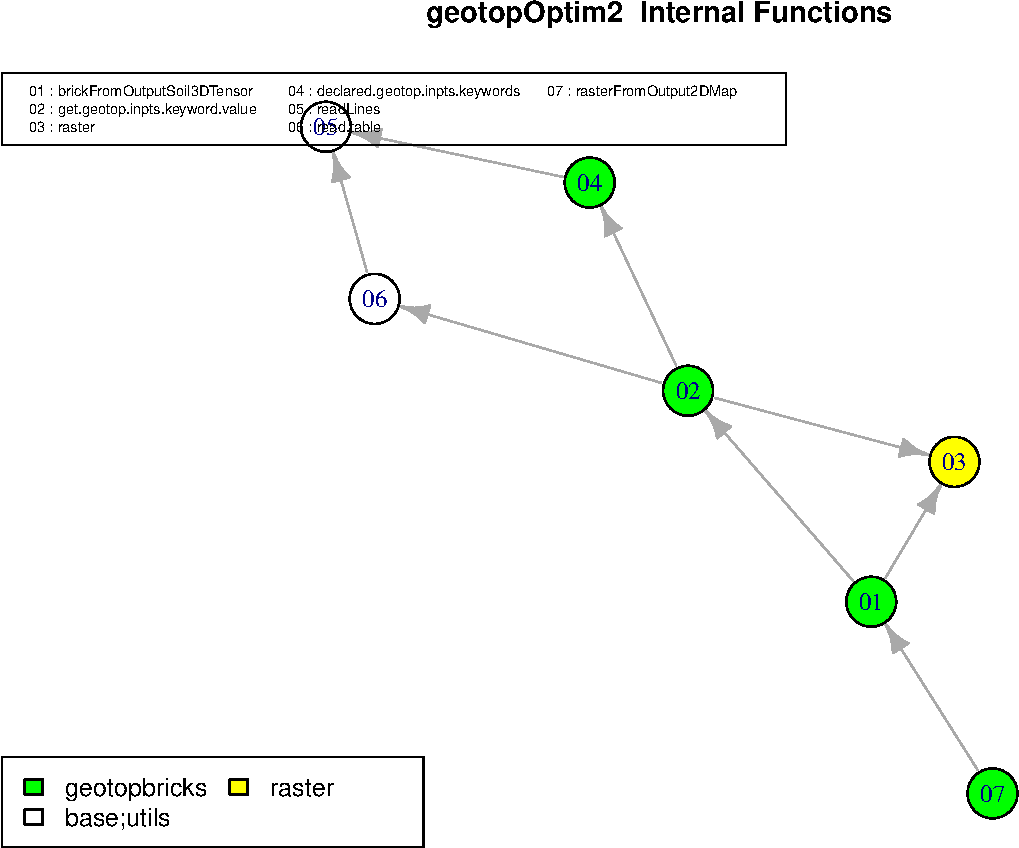
\includegraphics{presentation_files/figure-beamer/unnamed-chunk-1-1.pdf}

\end{frame}

\begin{frame}[fragile]{Simulation of soil water budget in an alpine
site}
\protect\hypertarget{simulation-of-soil-water-budget-in-an-alpine-site-1}{}

Here is the directory containing files of B2 point simulation:

\begin{Shaded}
\begin{Highlighting}[]
\KeywordTok{library}\NormalTok{(geotopbricks) }

\CommentTok{## SET GEOTOP WORKING DIRECTORY}
\NormalTok{wpath_B2 <-}\StringTok{ "resources/simulation/Matsch_B2_Ref_007"} 
\CommentTok{##writeLines(list.files(wpath_B2))}
\end{Highlighting}
\end{Shaded}

\end{frame}

\begin{frame}[fragile]{Getting simulation input data}
\protect\hypertarget{getting-simulation-input-data}{}

\begin{Shaded}
\begin{Highlighting}[]
\NormalTok{tz <-}\StringTok{ "Etc/GMT-1"}
\NormalTok{meteo <-}\StringTok{ }\KeywordTok{get.geotop.inpts.keyword.value}\NormalTok{(}
  \StringTok{"MeteoFile"}\NormalTok{,}
  \DataTypeTok{wpath=}\NormalTok{wpath_B2,}
  \DataTypeTok{data.frame=}\OtherTok{TRUE}\NormalTok{,}
  \DataTypeTok{tz=}\NormalTok{tz)}
\KeywordTok{head}\NormalTok{(meteo[}\DecValTok{12}\OperatorTok{:}\DecValTok{14}\NormalTok{,}\KeywordTok{c}\NormalTok{(}\StringTok{"Iprec"}\NormalTok{,}\StringTok{"WindSp"}\NormalTok{,}\StringTok{"WindDir"}\NormalTok{)])}
\end{Highlighting}
\end{Shaded}

\begin{verbatim}
##                     Iprec WindSp WindDir
## 2009-10-02 11:00:00     0   3.63  339.75
## 2009-10-02 12:00:00     0   2.75  328.48
## 2009-10-02 13:00:00     0   2.74  311.28
\end{verbatim}

\begin{Shaded}
\begin{Highlighting}[]
\KeywordTok{head}\NormalTok{(meteo[}\DecValTok{12}\OperatorTok{:}\DecValTok{14}\NormalTok{,}\KeywordTok{c}\NormalTok{(}\StringTok{"RelHum"}\NormalTok{,}\StringTok{"AirT"}\NormalTok{,}\StringTok{"Swglobal"}\NormalTok{)])}
\end{Highlighting}
\end{Shaded}

\begin{verbatim}
##                     RelHum  AirT Swglobal
## 2009-10-02 11:00:00  31.45 12.38   396.02
## 2009-10-02 12:00:00  30.50 13.12   500.07
## 2009-10-02 13:00:00  30.20 13.96   564.02
\end{verbatim}

\end{frame}

\begin{frame}[fragile]{Getting output simulation data}
\protect\hypertarget{getting-output-simulation-data}{}

Soil Water Content Profile:

\begin{Shaded}
\begin{Highlighting}[]
\NormalTok{tz <-}\StringTok{ "Etc/GMT-1"}
\NormalTok{SWC_B2  <-}\StringTok{ }\KeywordTok{get.geotop.inpts.keyword.value}\NormalTok{(}
  \StringTok{"SoilLiqContentProfileFile"}\NormalTok{,}
  \DataTypeTok{wpath =}\NormalTok{ wpath_B2,}
  \DataTypeTok{data.frame =} \OtherTok{TRUE}\NormalTok{,}
  \DataTypeTok{date_field =} \StringTok{"Date12.DDMMYYYYhhmm."}\NormalTok{,}
  \DataTypeTok{tz =}\NormalTok{ tz,}
  \DataTypeTok{zlayer.formatter =} \StringTok{"z%04d"}
\NormalTok{)}
\KeywordTok{help}\NormalTok{(get.geotop.inpts.keyword.value) }\CommentTok{## for more details!}
\end{Highlighting}
\end{Shaded}

\end{frame}

\begin{frame}[fragile]{P2}
\protect\hypertarget{p2}{}

The same for P2:

\begin{Shaded}
\begin{Highlighting}[]
\NormalTok{wpath_P2 <-}\StringTok{ "resources/simulation/Matsch_P2_Ref_007"} 
\NormalTok{SWC_P2  <-}\StringTok{ }\KeywordTok{get.geotop.inpts.keyword.value}\NormalTok{(}
  \StringTok{"SoilLiqContentProfileFile"}\NormalTok{,}
  \DataTypeTok{wpath =}\NormalTok{ wpath_P2,}
  \DataTypeTok{data.frame =} \OtherTok{TRUE}\NormalTok{,}
  \DataTypeTok{date_field =} \StringTok{"Date12.DDMMYYYYhhmm."}\NormalTok{,}
  \DataTypeTok{tz =} \StringTok{"Etc/GMT-1"}\NormalTok{,}
  \DataTypeTok{zlayer.formatter =} \StringTok{"z%04d"}\NormalTok{)}
\end{Highlighting}
\end{Shaded}

\end{frame}

\begin{frame}[fragile]{Data Reformatting}
\protect\hypertarget{data-reformatting}{}

\begin{Shaded}
\begin{Highlighting}[]
\KeywordTok{class}\NormalTok{(SWC_B2)}
\end{Highlighting}
\end{Shaded}

\begin{verbatim}
## [1] "zoo"
\end{verbatim}

\begin{Shaded}
\begin{Highlighting}[]
\NormalTok{SWC_B2 <-}\StringTok{ }\KeywordTok{cbind}\NormalTok{(}\DataTypeTok{time=}\KeywordTok{index}\NormalTok{(SWC_B2),}\KeywordTok{as.data.frame}\NormalTok{(SWC_B2))}
\KeywordTok{class}\NormalTok{(SWC_B2)}
\end{Highlighting}
\end{Shaded}

\begin{verbatim}
## [1] "data.frame"
\end{verbatim}

\begin{Shaded}
\begin{Highlighting}[]
\KeywordTok{names}\NormalTok{(SWC_B2)}
\end{Highlighting}
\end{Shaded}

\begin{verbatim}
##  [1] "time"  "z0001" "z0002" "z0003" "z0004" "z0006" "z0009" "z0013"
##  [9] "z0018" "z0023" "z0028" "z0035" "z0045" "z0055" "z0065" "z0078"
## [17] "z0093"
\end{verbatim}

\begin{Shaded}
\begin{Highlighting}[]
\CommentTok{###knitr::kable(head(SWC_B2))}
\end{Highlighting}
\end{Shaded}

\end{frame}

\begin{frame}{Stuff}
\protect\hypertarget{stuff}{}

Hydrological models are solvers of the differantial equations of water
flows and water thermodymanics in the Earth associated to heat transfers
between Earth and the low atmosphere. They are a simplification of a
real-world system useful to understand, predict, manage water resources.
''integrated''

\end{frame}

\begin{frame}[fragile]{Computation}
\protect\hypertarget{computation}{}

LOREM IPSUM:

\begin{itemize}
\item
  getting your data in the right shape (e.g. \texttt{tidyverse},
  \texttt{recipes})
\item
  getting your data in the right shape (e.g. \texttt{tidyverse},
  \texttt{recipes})
\item
  lorem ipsum
\end{itemize}

\end{frame}

\begin{frame}{Interested?}
\protect\hypertarget{interested}{}

www.geotop.org

Thank you for your attention! / Merci pour votre attention!

\end{frame}

\begin{frame}{Addendum}
\protect\hypertarget{addendum}{}

LOREM IPSUM

\end{frame}

\end{document}
